% =====================================================================
%  Supervisor presentation: covering-based robustness pre-process for CSLAP
%  Compile with pdfLaTeX in Overleaf. Standard packages only.
% =====================================================================
\documentclass[11pt,aspectratio=169]{beamer}
\usepackage[table]{xcolor}

\usetheme{Madrid}
\usecolortheme{default}
\setbeamertemplate{navigation symbols}{}
\setbeamertemplate{caption}[numbered]

\usepackage[utf8]{inputenc}
\usepackage[T1]{fontenc}
\usepackage{amsmath,amssymb}
\usepackage{booktabs}
\usepackage{tikz}
\usetikzlibrary{fit,backgrounds,positioning,arrows.meta}

\definecolor{accent}{RGB}{30,90,150}
\setbeamercolor{frametitle}{bg=accent,fg=white}
\setbeamercolor{title}{bg=accent,fg=white}
\setbeamercolor{block title}{bg=accent!18,fg=black}

\newcommand{\kk}{\kappa}

% --- Title -----------------------------------------------------------
\title[Robust covering pre-process for CSLAP]{A Covering-Based Pre-Process for Robust\\Storage Location Assignment}
\subtitle{Outer-approximating orders to hedge against demand shift}
% \author[Author]{Author Name}
% \institute[Affiliation]{Affiliation \\ \texttt{email@domain}}
% \date{\today}

\begin{document}

\begin{frame}[plain]
  \titlepage
\end{frame}

% --- Outline ---------------------------------------------------------
\begin{frame}{Table of Content}
  \begin{enumerate}
    \item The problem: handling uncertainty on future orders which are unknown.
    \item The idea: enlarge the orders \emph{before} optimizing.
    \item The model: a min--max covering partition.
    \item The knob $\kk$: how cautious do we choose to be?
    \item What we count vs.\ what we optimize.
    \item Results.
  \end{enumerate}
\end{frame}

% =====================================================================
\section{Motivation}
% =====================================================================
\begin{frame}{The problem we are addressing}
  \begin{block}{Correlated Storage Location Assignment (CSLAP)}
    Place each SKU at a picking station so that an order is collected from as
    \alert{few stations} as possible. Products that are ordered together should
    sit together.
  \end{block}
  \vspace{0.5em}
  \begin{itemize}
    \item A layout is fitted on a window of \alert{past orders}, then operated
          for weeks or months.
    \item During operation, the order mix \alert{drifts}: new product
          combinations appear, old ones fade.
    \item A layout tuned \emph{exactly} to past orders can age badly. It is
          optimal for a demand that no longer exists.
  \end{itemize}
  \vspace{0.5em}
  \begin{center}
    \emph{Question: can we make the layout more durable by optimizing on a
    deliberately broader picture of demand?}
  \end{center}
\end{frame}

\begin{frame}{Our hypothesis}
  \begin{alertblock}{H1}
    A layout optimized on a deliberately \textbf{enlarged} demand object is more
    robust to future order-distribution shift than one optimized directly on the
    observed orders --- at a bounded nominal cost.
  \end{alertblock}
  \vspace{0.6em}
  % \begin{itemize}
  %   \item We test H1; we do not assume it.
  %   \item We report the upside \emph{and} the cost, and we report where it fails.
  %   \item A partial or negative result is a valid scientific outcome.
  % \end{itemize}
\end{frame}

% =====================================================================
\section{The idea}
% =====================================================================
\begin{frame}{The idea in one picture}
  \begin{center}
  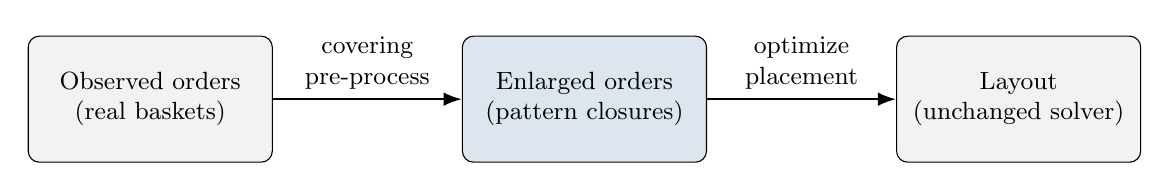
\begin{tikzpicture}[font=\small,>=Latex]
    \node[draw,rounded corners,fill=gray!10,minimum width=3.1cm,minimum height=1.6cm,align=center]
      (raw) {Observed orders\\(real baskets)};
    \node[draw,rounded corners,fill=accent!15,minimum width=3.1cm,minimum height=1.6cm,align=center,right=2.4cm of raw]
      (big) {Enlarged orders\\(pattern closures)};
    \node[draw,rounded corners,fill=gray!10,minimum width=3.1cm,minimum height=1.6cm,align=center,right=2.4cm of big]
      (lay) {Layout\\(unchanged solver)};
    \draw[->,thick] (raw) -- node[above,align=center]{covering\\pre-process} (big);
    \draw[->,thick] (big) -- node[above,align=center]{optimize\\placement} (lay);
  \end{tikzpicture}
  \end{center}
  \vspace{0.4em}
  \begin{itemize}
    \item A \alert{pre-process} sits in front of the existing pipeline.
    \item It widens each order to include closely co-ordered companions.
    \item The placement solvers run \alert{unchanged} on the wider orders.
    \item Nothing inside the optimization model is rewritten.
  \end{itemize}
\end{frame}

\begin{frame}{What the pre-process does}
  \begin{enumerate}
    \item Group SKUs into \alert{bundles} (patterns) of co-ordered products,
          each of size at most $\kk$. The bundles \alert{tile} the whole
          catalogue: every SKU sits in exactly one bundle.
    \item Replace each order by its \alert{closure}: the union of every bundle
          it touches.
    \item Hand the enlarged orders to the existing solver.
  \end{enumerate}
  \vspace{0.6em}
  % \begin{block}{Plain reading}
  %   ``If you ordered B and C, and our bundles say B travels with A and C travels
  %   with D, then optimize as if A and D came too.'' The layout is then forced to
  %   keep these neighbourhoods together --- even for combinations no customer has
  %   literally ordered yet.
  % \end{block}
\end{frame}

% =====================================================================
\section{The model}
% =====================================================================
\begin{frame}{The covering model (the pre-process, as an optimization)}
  Pick a tiling of the catalogue into bundles so that no order is scattered
  across too many bundles.
  \begin{align*}
    \min_{x,\,\Pi}\quad & \Pi \\
    \text{s.t.}\quad
      & \sum_{q \ni p} x_q = 1 && \forall\, p \in P \\
      & \sum_{q:\, q \cap P_o \neq \emptyset} x_q \le \Pi && \forall\, o \in O^{tr}_{\neq} \\
      & x_q \in \{0,1\}, \quad \Pi \ge 0, \quad |q|\le \kk
  \end{align*}
  \begin{itemize}\small
    \item \textbf{Objective:} minimize $\Pi$, the spread of the \emph{worst} order
          (a min--max bottleneck).
    \item \textbf{First constraint:} each SKU lands in exactly one bundle (a partition).
    \item \textbf{Second constraint:} no order touches more than $\Pi$ bundles.
  \end{itemize}
\end{frame}

\begin{frame}{Notation at a glance}
  \begin{center}
  \begin{tabular}{@{}ll@{}}
    \toprule
    Symbol & Meaning \\
    \midrule
    $P$ & universe of SKUs (the whole catalogue) \\
    $O^{tr}$, $P_o$ & training orders; SKUs in order $o$ \\
    $O^{tr}_{\neq}$ & distinct order contents (one constraint each) \\
    $q \in Q$ & a bundle (pattern) of co-ordered SKUs \\
    $\kk$ & maximum bundle size --- the conservatism knob \\
    $x_q \in \{0,1\}$ & keep bundle $q$ in the tiling? \\
    $\Pi \ge 0$ & worst order's bundle-spread (minimized) \\
    $\bar P_o$ & closure of order $o$ (its enlarged basket) \\
    \bottomrule
  \end{tabular}
  \end{center}
  \vspace{0.6em}
  \begin{block}{The solving engine (one line)}
    Bundles are never listed exhaustively. \alert{Column generation} invents
    promising bundles on demand through a pricing subproblem of size $\le \kk$.
  \end{block}
\end{frame}

\begin{frame}{From bundles to the enlarged order}
  Once the tiling is fixed, each order is enlarged to its closure:
  \[
    \bar P_o \;=\; \bigcup_{\,q\,:\, q \cap P_o \neq \emptyset} q
    \qquad\text{(union of every bundle the order touches).}
  \]
  \begin{itemize}
    \item The closure always \alert{contains} the real order: $P_o \subseteq \bar P_o$.
    \item So the enlarged set is an \alert{outer approximation} of the observed demand.
    \item Enlarging is the \emph{conservative} direction: we optimize against
          more order-shapes than we literally saw.
  \end{itemize}
\end{frame}

% =====================================================================
\section{Worked example}
% =====================================================================
\begin{frame}{A small example you can picture}
  Six real SKUs from the dataset, relabelled A--F for readability:
  \begin{center}\small
    A\,=1000270,\quad B\,=1000290,\quad C\,=1000295,\\
    D\,=1000296,\quad E\,=1000361,\quad F\,=1000364
  \end{center}
  Five observed orders, each a neighbouring pair (a co-occurrence chain):
  \[
    O_1=\{A,B\}\quad O_2=\{B,C\}\quad O_3=\{C,D\}\quad O_4=\{D,E\}\quad O_5=\{E,F\}
  \]
  % \begin{center}
  % \begin{tikzpicture}[font=\small]
  %   \foreach \n/\x in {A/0,B/1.4,C/2.8,D/4.2,E/5.6,F/7.0}{\node (\n) at (\x,0) {\n};}
  %   \foreach \a/\b in {A/B,B/C,C/D,D/E,E/F}{\draw[gray] (\a)--(\b);}
  % \end{tikzpicture}\\[-0.2em]
  % {\footnotesize lines = pairs that were ordered together}
  % \end{center}
\end{frame}

\begin{frame}{$\kk=1$: no enlargement (the baseline / direct method)}
  Bundles must be singletons: \{A\}\,\{B\}\,\{C\}\,\{D\}\,\{E\}\,\{F\}.
  Each order touches only its own SKUs $\Rightarrow$ closure = order.
  \begin{center}
  \begin{tabular}{@{}lccc@{}}
    \toprule
    Order & bundles touched & closure $\bar P_o$ & size \\
    \midrule
    $O_1=\{A,B\}$ & \{A\},\{B\} & \{A,B\} & 2 \\
    $O_2=\{B,C\}$ & \{B\},\{C\} & \{B,C\} & 2 \\
    $O_3=\{C,D\}$ & \{C\},\{D\} & \{C,D\} & 2 \\
    $O_4=\{D,E\}$ & \{D\},\{E\} & \{D,E\} & 2 \\
    $O_5=\{E,F\}$ & \{E\},\{F\} & \{E,F\} & 2 \\
    \bottomrule
  \end{tabular}
  \end{center}
  \vspace{0.4em}
  Mean closure $=2.0$, enlargement ratio $\bar c = 1.0$. This is exactly the
  classic ``feed the raw orders'' approach.
\end{frame}

\begin{frame}{$\kk=2$: bundles of two}
  A tiling: \fbox{A\,B}\ \ \fbox{C\,D}\ \ \fbox{E\,F}.
  % \begin{center}
  % \begin{tikzpicture}[font=\small]
  %   \foreach \n/\x in {A/0,B/1.4,C/2.8,D/4.2,E/5.6,F/7.0}{\node (\n) at (\x,0) {\n};}
  %   \begin{scope}[on background layer]
  %     \node[draw,rounded corners,fill=accent!15,fit=(A)(B),inner sep=4pt]{};
  %     \node[draw,rounded corners,fill=green!18,fit=(C)(D),inner sep=4pt]{};
  %     \node[draw,rounded corners,fill=orange!20,fit=(E)(F),inner sep=4pt]{};
  %   \end{scope}
  % \end{tikzpicture}
  % \end{center}
  \begin{center}\small
  \begin{tabular}{@{}lccc@{}}
    \toprule
    Order & bundles touched & closure $\bar P_o$ & size \\
    \midrule
    $O_1=\{A,B\}$ & \fbox{AB} & \{A,B\} & 2 \\
    $O_2=\{B,C\}$ & \fbox{AB}\,\fbox{CD} & \alert{\{A,B,C,D\}} & 4 \\
    $O_3=\{C,D\}$ & \fbox{CD} & \{C,D\} & 2 \\
    $O_4=\{D,E\}$ & \fbox{CD}\,\fbox{EF} & \alert{\{C,D,E,F\}} & 4 \\
    $O_5=\{E,F\}$ & \fbox{EF} & \{E,F\} & 2 \\
    \bottomrule
  \end{tabular}
  \end{center}
  Mean closure $=2.8$, $\bar c = 1.4$. Orders on a seam (e.g.\ $O_2$) inflate.
\end{frame}

\begin{frame}{$\kk=3$: bundles of three}
  A tiling: \fbox{A\,B\,C}\ \ \fbox{D\,E\,F}.
  \begin{center}\small
  \begin{tabular}{@{}lccc@{}}
    \toprule
    Order & bundles touched & closure $\bar P_o$ & size \\
    \midrule
    $O_1=\{A,B\}$ & \fbox{ABC} & \{A,B,C\} & 3 \\
    $O_2=\{B,C\}$ & \fbox{ABC} & \{A,B,C\} & 3 \\
    $O_3=\{C,D\}$ & \fbox{ABC}\,\fbox{DEF} & \alert{\{A,B,C,D,E,F\}} & 6 \\
    $O_4=\{D,E\}$ & \fbox{DEF} & \{D,E,F\} & 3 \\
    $O_5=\{E,F\}$ & \fbox{DEF} & \{D,E,F\} & 3 \\
    \bottomrule
  \end{tabular}
  \end{center}
  \vspace{0.3em}
  Mean closure $=3.6$, $\bar c = 1.8$.
  \begin{block}{The trend}
    $\bar c:\ 1.0 \;\to\; 1.4 \;\to\; 1.8$ as $\kk$ grows. Bigger bundles $\Rightarrow$
    bigger enlarged orders $\Rightarrow$ a wider hedge.
    \footnotesize(On the real data: synthetic $\bar c \approx 1.0\!\to\!1.75\!\to\!2.2$; industrial $\approx 1.0\!\to\!1.33\!\to\!1.57$.)
  \end{block}
\end{frame}

% =====================================================================
\section{The knob}
% =====================================================================
\begin{frame}{$\kk$ is the conservatism dial}
  \begin{center}
  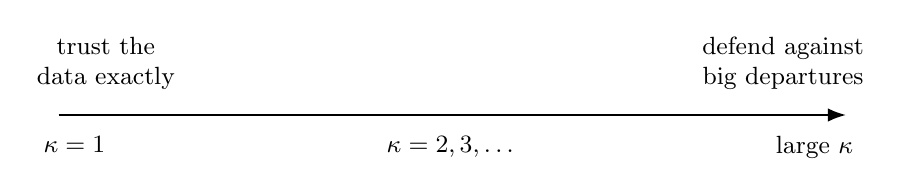
\begin{tikzpicture}[font=\small,>=Latex]
    \draw[->,thick] (0,0) -- (10,0);
    \node[below] at (0.2,-0.15) {$\kk=1$};
    \node[below] at (5,-0.15) {$\kk=2,3,\dots$};
    \node[below] at (9.6,-0.15) {large $\kk$};
    \node[above,align=center] at (0.6,0.2) {trust the\\data exactly};
    \node[above,align=center] at (9.2,0.2) {defend against\\big departures};
  \end{tikzpicture}
  \end{center}
  \vspace{0.3em}
  \begin{itemize}
    \item $\kk=1$: zero enlargement, optimize on what you saw (cheap, fragile).
    \item Larger $\kk$: coarser bundles, larger closures, more caution
          (safer, costlier on the nominal orders).
  \end{itemize}
  \begin{alertblock}{Concept}
    $\kk$ plays the role of the single dial in robust
    optimization: the budget $\Gamma$ of Bertsimas \& Sim, or the ambiguity
    radius in distributionally robust optimization.
  \end{alertblock}
\end{frame}

% =====================================================================
\section{Why it is robust optimization}
% =====================================================================
\begin{frame}{This is robust optimization}
  \begin{block}{Result (stated plainly)}
    Optimizing visits on the enlarged orders is \alert{identical} to solving a
    robust counterpart of CSLAP, where each order may be \emph{any} sub-basket of
    its closure:
    \[
      \min_{a}\ \sum_{o} v\!\left(a,\bar P_o\right)
      \;=\;
      \min_{a}\ \sum_{o}\ \max_{u\,\subseteq\,\bar P_o} v\!\left(a,u\right).
    \]
  \end{block}
  \begin{itemize}
    \item $v(a,u)$ = number of stations order $u$ visits under layout $a$.
    \item Adding products can only add visits, so the worst case is the full
          closure $\Rightarrow$ the inner ``adversary'' is trivial.
    % \item That is \emph{why} the unchanged solvers already solve the robust problem.
  \end{itemize}
  \vspace{0.3em}
  {\footnotesize The uncertainty set is \emph{learned from data} via the cover ---
  in the spirit of data-driven uncertainty-set design. What stays a hypothesis
  (H1) is that future orders actually fall inside it.}
\end{frame}

% =====================================================================
\section{What we count}
% =====================================================================
\begin{frame}{We enlarge to place --- but we count on real demand}
  \begin{center}
  \begin{tabular}{@{}lll@{}}
    \toprule
    Phase & Sees & Produces \\
    \midrule
    Optimize & \alert{enlarged} orders $\bar P_o$ & the layout $a$ \\
    Count / score & \alert{real} orders $P_o$ only & the reported visit numbers \\
    \bottomrule
  \end{tabular}
  \end{center}
  \vspace{0.6em}
  \begin{itemize}
    \item Every reported figure (training cost \emph{and} test cost) is counted on
          \alert{real baskets}. The closures are discarded before counting.
    % \item A product placed near its bundle still scores a visit \emph{only} in
    %       orders that truly contain it. The synthetic demand never inflates the tally.
    % \item The direct ($\kk=1$) layout and the robust ($\kk\!\ge\!2$) layout are
    %       scored on the \alert{same real orders} --- one identical yardstick.
  \end{itemize}
  \vspace{0.3em}
  {\footnotesize Enlargement changes \emph{where} products go, not \emph{what} we measure.}
\end{frame}

% =====================================================================
\section{Results}
% =====================================================================
\begin{frame}{Evaluation set-up}
  \begin{itemize}
    \item Build the layout on \alert{training} orders only; score on \alert{held-out}
          orders. Strict no-leakage (construction never sees test data).
    % \item Two shift sources: a \alert{synthetic} order-shift family (graded
    %       distribution change, 45 cells, 3 training seeds) and one \alert{industrial}
    %       temporal hold-out (early weeks $\to$ later weeks).
    \item One \alert{industrial} temporal hold-out (early weeks $\to$ later weeks).
    \item Two headline numbers, robust layout vs.\ nominal layout:
  \end{itemize}
  \vspace{0.4em}
  \begin{center}
  \begin{tabular}{@{}ll@{}}
    \toprule
    Price of robustness, $\mathrm{PoR}$ & extra cost on the \emph{training} orders \\
    Out-of-sample gain, $G$ & savings on the \emph{future} orders  \\
    \bottomrule
  \end{tabular}
  \end{center}
\end{frame}

% \begin{frame}{Synthetic result: a stable price, an unstable gain}
%   \begin{itemize}
%     \item \alert{Price is real and stable}: positive in all 18 genuine cells
%           (rises with $\kk$). The cost side behaves exactly as the theory predicts.
%     \item \alert{Gain does not replicate} across training seeds, with one exception.
%   \end{itemize}
%   \begin{center}\small
%   \begin{tabular}{@{}llccc@{}}
%     \toprule
%     Solver & $\kk$ & gain $G$ across seeds & pooled $p$ & verdict \\
%     \midrule
%     Genetic alg.\ & 2 & $+\,/\,+\,/\,+$ & \textbf{0.003} & \alert{replicated} (+0.58\%) \\
%     Heuristic & 2 & $+\,/\,-\,/\,+$ & 0.48 & not stable \\
%     Sim.\ annealing & 2 & $+\,/\,-\,/\,-$ & 0.14 & not stable \\
%     \bottomrule
%   \end{tabular}
%   \end{center}
%   \vspace{0.4em}
%   \begin{itemize}\footnotesize
%     \item Only the genetic-algorithm layout at $\kk=2$ gains consistently
%           (mean $+0.58\%$, 95\% CI $[+0.18,+0.98]$).
%     \item No global directional effect (11/18 cells positive, sign-test $p=0.48$);
%           the predicted ``sweet spot'' in $\kk$ does not appear.
%   \end{itemize}
% \end{frame}

\begin{frame}{Industrial result}
  One real temporal hold-out (219k train / 66k test orders, 21k SKUs).
  Only the greedy heuristic both scaled and produced distinct layouts.
  \begin{center}\small
  \begin{tabular}{@{}lccc@{}}
    \toprule
    $\kk$ & price on train & gain on future orders \\
    \midrule
    2 & $-0.9\%$ & $+0.3\%$ \\
    3 & $-2.5\%$ & $+2.0\%$ \\
    \bottomrule
  \end{tabular}
  \end{center}
  \vspace{0.4em}
  \begin{itemize}
    \item Here the robust layout improved \emph{both} train and future visits.
    % \item This is \alert{not} a free lunch: the greedy solver is sub-optimal, and
    %       the enlarged orders simply guide it to a better real-objective layout.
    %       Leakage excluded (disjoint temporal split; construction sees train only).
    % \item Caveat: a \alert{single} test cell (no confidence interval); the other
    %       two solvers did not scale / did not differentiate.
    \item The only test we could conduct was with the greedy heuristic for scale reasons
    \item Next step check all the other approaches we consider, like GA, SA, MILP, through a commercial solver
  \end{itemize}
\end{frame}

\begin{frame}{Workload check}
  \begin{center}\footnotesize
  \begin{tabular}{@{}rrrrrr@{}}
    \toprule
    \multicolumn{2}{c}{} & \multicolumn{2}{c}{$\kk=1$ (nominal)} & \multicolumn{2}{c}{$\kk=2$ (robust)}\\
    \cmidrule(lr){3-4}\cmidrule(lr){5-6}
    St & real $T_s$ & $W_s$ & \%$T_s$ & $W_s$ & \%$T_s$ \\
    \midrule
    \rowcolor{red!10}
    1  & 495   & 8063 & \textcolor{red}{\textbf{1629\%}} & 8753 & \textcolor{red}{\textbf{1768\%}} \\
    2  & 3582  & 8196 & \textcolor{red}{229\%}           & 7550 & \textcolor{red}{211\%}           \\
    3  & 1935  & 2752 & \textcolor{red}{142\%}           & 2866 & \textcolor{red}{148\%}           \\
    4  & 2570  & 2557 & 99\%  & 2467 & 96\% \\
    5  & 2816  & 2642 & 94\%  & 2391 & 85\% \\
    22 & 1870  & 1801 & 96\%  & 1727 & 92\% \\
    23 & 9524  & 6404 & 67\%  & 6325 & 66\% \\
    24 & 6778  & 2698 & 40\%  & 2636 & 39\% \\
    \bottomrule
  \end{tabular}\\[+0.8em]
  {\scriptsize Stations 6--21 and 25 are all under 50\% load in both arms (omitted). $W_s = \sum_{p\to s} L_p / V_s$.}
  \end{center}
  % \vspace{0.2em}
  % \begin{alertblock}{Reading}
  %   \footnotesize
  %   \begin{itemize}
  %     \item Both arms \alert{already} break the real workload cap on stations 1--3;
  %           station 1 sits $\sim$16$\times$ over (slot-rich, time-poor).
  %     \item $\kk=2$ does not relieve it and nudges the worst station up
  %           ($1629\% \!\to\! 1768\%$); it is a redistribution, not a uniform worsening.
  %     \item The heuristic enforces \emph{slots only}, not workload, so it overloads
  %           station~1; an exact solver would not. The BERNER saving is a
  %           \alert{visits-only} result.
  %   \end{itemize}
  % \end{alertblock}
\end{frame}


\begin{frame}{Honest limitations}
  \begin{itemize}
    \item \textbf{No exact solver ran.} Gurobi/CPLEX were unavailable; the open
          solver forced a sub-sample, so the certified bottleneck $\Pi$ is local,
          not global ($34$ on the sample vs.\ $369$ on the full stream).
    \item \textbf{Capacity recalibration confound.} Enlarging inflates apparent
          workload; loosening the capacity constraint 
          %mixes two effects in the numbers (documented, measured).
    \item \textbf{Narrow industrial evidence.} One temporal cell, one solver.
    \item \textbf{Gain is small} because our current industrial data does not drift much in the future.
  \end{itemize}
  % \vspace{0.3em}
  % \begin{block}{Reported as a contribution}
  %   The non-replication is a finding, not a failure: it tells us \emph{when} the
  %   pre-process pays off and when it does not.
  % \end{block}
\end{frame}

% =====================================================================
\section{Takeaways}
% =====================================================================
\begin{frame}{What we achieved}
  \begin{enumerate}
    \item A \alert{pre-process} that turns CSLAP placement into a data-driven
          \alert{robust counterpart} --- with an exact equivalence, not an analogy.
    \item It reuses every existing solver \alert{unchanged}; the only new object
          is the covering construction.
    \item A single tunable knob $\kk$ for the price/robustness trade-off.
    % \item A leakage-free evaluation, honest about what counts and what does not.
    % \item A clear, mixed verdict: \alert{stable price, conditional gain}.
  \end{enumerate}
\end{frame}

\begin{frame}{Next steps}
  \begin{itemize}
    \item \alert{Exact solver at scale} (Gurobi/CPLEX): certify the true $\Pi$,
          run the full cover without sub-sampling, and observe the price-of-robustness
          where the theory bites (at optimality).
    % \item A scalable simulated-annealing objective to restore a second
    %       metaheuristic on the industrial instance.
    % \item Several temporal cuts and several industrial sites, to attach
    %       dispersion to the industrial gain.
    \item Test on synthetic datasets
  \end{itemize}
  \vspace{0.6em}
  \begin{center}
    \emph{The construction is sound and reusable}
    %; the robustness payoff at this scale is conditional --- and we now know on what.}
  \end{center}
\end{frame}

% =====================================================================
\section*{References}
% =====================================================================
\begin{frame}[allowframebreaks]{Selected references}
  \footnotesize
  \begin{thebibliography}{99}
    \bibitem{bertsimas2004} Bertsimas, D., Sim, M.\ (2004). The price of robustness. \emph{Operations Research} 52(1), 35--53.
    \bibitem{bbc2011} Bertsimas, D., Brown, D.B., Caramanis, C.\ (2011). Theory and applications of robust optimization. \emph{SIAM Review} 53(3), 464--501.
    \bibitem{esfahani2018} Mohajerin Esfahani, P., Kuhn, D.\ (2018). Data-driven distributionally robust optimization using the Wasserstein metric. \emph{Mathematical Programming} 171, 115--166.
    \bibitem{bgk2018} Bertsimas, D., Gupta, V., Kallus, N.\ (2018). Data-driven robust optimization. \emph{Mathematical Programming} 167(2), 235--292.
    \bibitem{balas1976} Balas, E., Padberg, M.W.\ (1976). Set partitioning: a survey. \emph{SIAM Review} 18(4), 710--760.
    \bibitem{dekoster2007} de Koster, R., Le-Duc, T., Roodbergen, K.J.\ (2007). Design and control of warehouse order picking: a literature review. \emph{EJOR} 182(2), 481--501.
    \bibitem{reyes2019} Reyes, J.J.R., Solano-Charris, E.L., Montoya-Torres, J.R.\ (2019). The storage location assignment problem: a literature review. \emph{IJIEC} 10(2), 199--224.
    \bibitem{mantel2007} Mantel, R.J., Schuur, P.C., Heragu, S.S.\ (2007). Order oriented slotting. \emph{EJIE} 1(3), 301--316.
    \bibitem{xiao2012} Xiao, J., Zheng, L.\ (2012). Correlated storage assignment to minimize zone visits for BOM picking. \emph{IJAMT} 61, 797--807.
    \bibitem{zhang2019} Zhang, R.-Q., Wang, M., Pan, X.\ (2019). New model of the SLAP considering demand correlation pattern. \emph{Computers \& Industrial Engineering} 129, 210--219.
    \bibitem{kofler2014} Kofler, M., Beham, A., Wagner, S., Affenzeller, M.\ (2014). Affinity based slotting in warehouses with dynamic order patterns. Springer, TIEI vol.\ 6, 123--143.
    \bibitem{gademann2005} Gademann, N., van de Velde, S.\ (2005). Order batching to minimize total travel time. \emph{IIE Transactions} 37(1), 63--75.
  \end{thebibliography}
\end{frame}

\begin{frame}[plain]
  \centering
  \vfill
  {\Large Thank you}\\[0.5em]
  {\normalsize Questions \& discussion}
  \vfill
\end{frame}

\end{document}
